\section{Approach}
In this part, we will present two parts of our work. The first one is about how to process the log file and get what kinds of information. The work flow of automatic dependency analysis is illustrated in Figure\ref{fig:steps}.
%\lipsum[1-2]
%\begin{wrapfigure}{R}{0.5\textwidth}
%	\begin{center}
%		\begin{adjustbox}{width=0.5\textwidth}
%			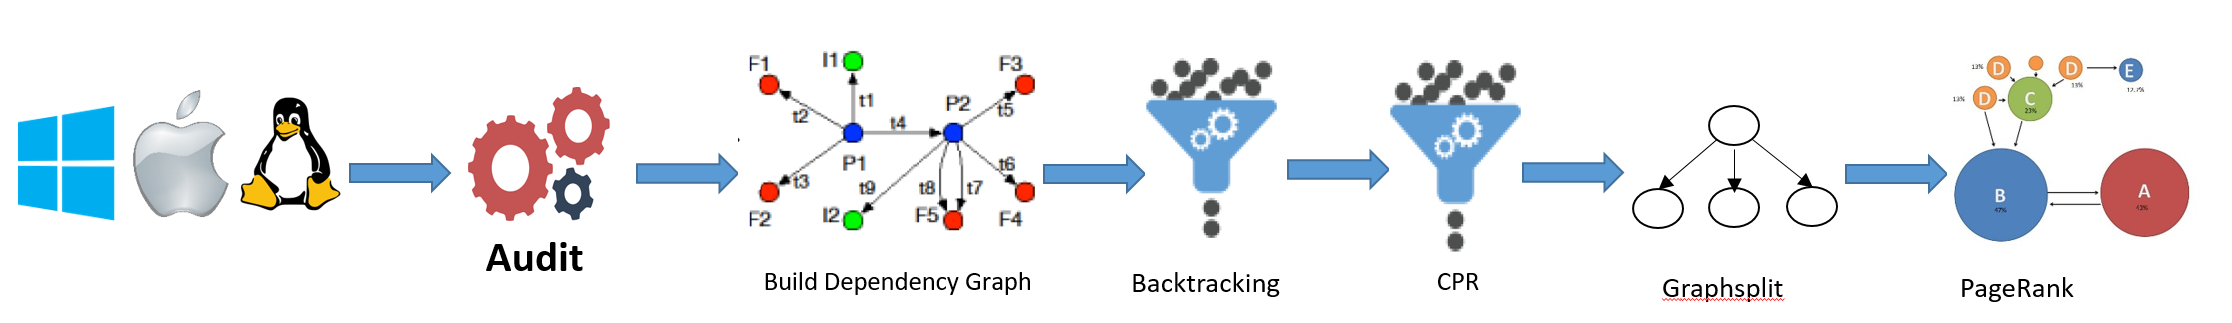
\includegraphics[clip,scale=0.35]{figFlow.png}
%		\end{adjustbox}
%	\end{center}
%\end{wrapfigure}
\begin{figure}[!htp]
	\centering

	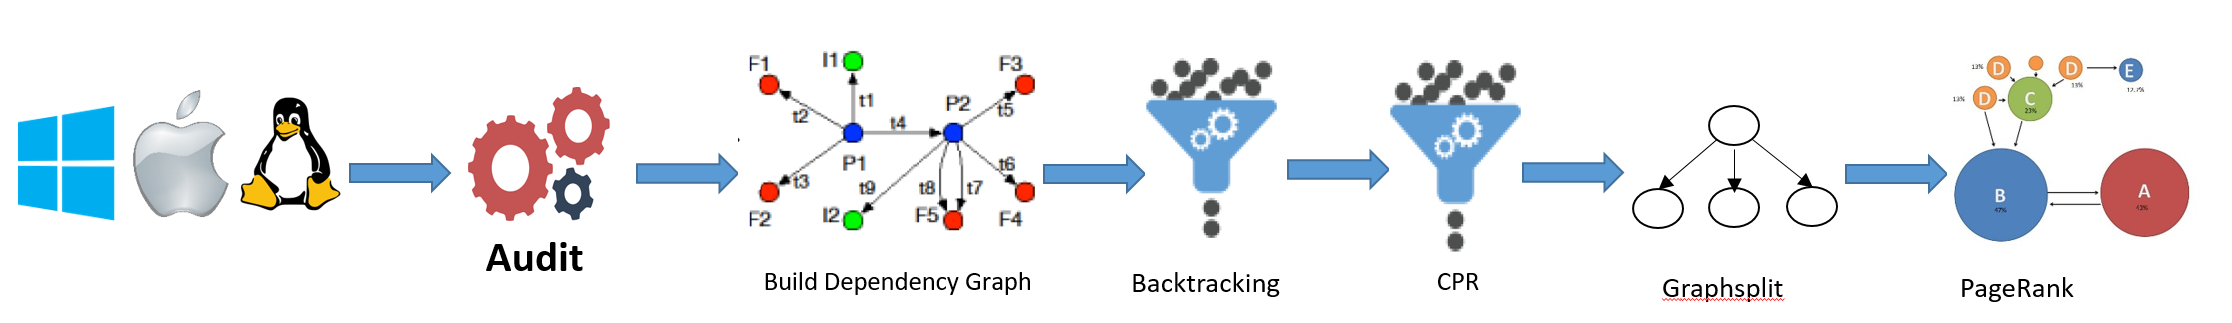
\includegraphics[width=0.48\textwidth]{figFlow.png}
	\caption{Overview of automatic dependency analysis}
	\label{fig:steps}
\end{figure}

\subsection{Enhanced Dependency Analysis (Milestone 1)}
In this section, we describe the 


\textbf{Log Parsing}.
After gathering the data, we need build the dependency graph based on the log file. There are three type vertexes representing three kind system entities: process, file and network communication.
The identifier for process is its name and id.  For file, it is identified by its absolute file path, for network communication, it is distinguished by the communication two sides' ip and port number.The attributes for these three system entities are showed in Table~\ref{mytable:table1}. We use three kind shape to represent these three system entities. According to the entities included in the system event, the parser need to process five kinds edge : process to process, process to file, file to process, network to process, process to network. The type of edge is decided by the event arguments. The output of Sysdig will use \textit{fd} as its identifier or key word. In the value part, it will use different characters to represent different objects.For example, it use \textit{f} to represent file, \textit{6} to represent IPV6 sockets,\textit{4} to represent IPV4 sockets. This kind information is necessary, without this, it is hard to know the start or end of information flow is a file or an ip address.  Through this way, the parser can know the kind of entities generating this event. For process to process event, we can directly know objects generating this event is two processes, because its event type is unique : fork or clone. In the conclusion, the parser will establish the dependency relationship between two system entities. This dependency relationship is specified by three parts: a source object, a sink object and a time interval$(t_s(e), t_e(e))$.Table2 shows the information that we collect in the log file.

\begin{table}[t!p]
	\centering
	\caption{Representation Of System Entities}
	\label{mytable:table1}
	\resizebox{0.45\textwidth}{!}{%
		\begin{tabular}{|l|c|r|}
			\hline
			Entity             & Attributes    & Shape in Graph \\ \hline
			File               & Absolute Path & Ellipse        \\ \hline
			Process            & PID and Name  & Square         \\ \hline
			Network Connection & IP and Port   & Parallelogram  \\ \hline
		\end{tabular}%
	}
\end{table}
\begin{table}[!htp]
	\centering
	\caption{Representative attributes of system events}
	\label{table2}
	\begin{tabular}{|l|c|}
		\hline
		Categories    & Attributes                    \\ \hline
		Operation     & read/write writeto fork clone \\ \hline
		Time/Sequence & Start/End Time                \\ \hline
		Argument      & IP Port data size             \\ \hline
	\end{tabular}
\end{table}




\textbf{Limitations of Existing Work}.
In the existed research work, the information for the dependency analysis only includes file name, process, IP addresses and attributes of events including event origins, operations $($file read/write$)$, and other security-related properties. However, to infer application reputation, only these attributes are not enough.
The reason is that they are mainly used to form a dependency graph with nodes being entities and edges representing data flows;
but to infer reputations, each edge carries different weights in impacting the reputation propagation as shown in Figure~\ref{fig:steps}.
Moreover, dependency analysis includes filters based on the existing works~\cite{backtracking,backtracking2}, which are not optimized for inferring reputations.
Therefore, it is \emph{necessary} to collect more attributes for the purpose of assigning weights to edges in the produced dependency graph and include more specialized filters to filter out unrelated events in the graph. 

\textbf{Relative Time to the POI event}.
Currently, we finished the building the dependency graph with additional necessary information. The first one is the relative time to the POI event(Detection Point).Once an application or a library is introduced to a system, it may get modifications via application updates, manually customizations, or malicious alternations. 
That is, a file node in the dependency graph can have multiple \emph{write} edges $($incoming edges$)$ representing initial creation and subsequent updates.
Intuitively, the write comes latter carries more weights in impacting the application reputation.
%For example, an application could be created by a benign program and latter gets altered by a malicious program; to capture the latter malicious alternation, usually injecting malicious code, the application's reputation should be considered as \emph{more towards malicious}. 
Therefore, \emph{the time when an event occurs} is one factor that impacts the reputation propagation: the latter it happens, the more weight it carries.
As such, given a POI event, we propose to compute \emph{the relative time to the start time of the POI event} for each of the subsequent edges included into the dependency graph,
and use this new attribute as part of the computation for the weights of the edges. 

\textbf{Amount of Transfered Data}.
The second  improvement compared with the traditional dependency analysis method is that we observe that the amount of transferred data is another important factor that impacts the reputation propagation.Not all the updates are rewriting application executables to malicious executables; some updates to an application are merely for property updates.
For example, in Windows, the search indexer program frequently updates executables' metadata for indexing purposes, and each update writes only a few bytes to the executables.
Therefore, we propose to extract \emph{the amount of data transferred} for each read/write operation and annotates the corresponding edges in the dependency graph with this information.
The larger amount of data transferred, the more important the edge is. So for the weight calculation, we need to consider the relative time and amount of data together. 
\begin{algorithm}[tb]
	\caption{GraphSplit}
	\KwIn{A dependency Graph}
	\SetKwFunction{FindPair}{FindPair}
	\SetKwFunction{UpdateGraph}{UpdateGraph}
	\SetKwFunction{RecoverTimeLogic}{RecoverTimeLogic}
	\textbf{function}: GraphSplit$(\textit(G))$\\
	$Queue$ $\leftarrow$ \FindPair{$G$}\;
	\While{Queue is not Empty}{
		$V$ $\leftarrow$ $Queue.poll()$\;
		$S \leftarrow V.source$\;
		$T \leftarrow V.target$\;
		\If{Set contains S $or$ Set contains T}{continue}
		$list1 \leftarrow$ list of outgoing edges of $S$ whose object is not $T$\;
		$list2 \leftarrow$ V.list\;
		\UpdateGraph($G$,$list1$,$list2$)\;
		add $S$ to Set\;
		$Queue \leftarrow$ \FindPair($G$)\;
	}
	\RecoverTimeLogic{$Set$}\;	
	\label{alg:split}
\end{algorithm}
\begin{algorithm}[!htbp]
	\caption{FindPair}
	\KwIn{A dependency Graph(G)}
	\KwResult{A queue containing the vertex pair need to be splited}
	\textbf{function}: FindPair$\textit(G)$\\
	$V \leftarrow G.vertexSet$\;
	\For{$v \in V$}{
		$E \leftarrow$ incoming edges of $v$\;
		\If{$\exists e \in E$ sharing the same source}{
			$vertexPair.source \leftarrow e.source$\;
			$vertextPair.object \leftarrow v$\;
			$vertexPair.object.list$ add $e$\; 
			$Queue$ add $vertexPair$\;}
	}
	\Return{Queue}
	\label{alg:find}
\end{algorithm}



\begin{table*}[!hp]
	\centering
	\caption{Statistical Result}
	\label{my-label}
	%	\resizebox{0.5\textwidth}{!}{%
	\begin{scriptsize}
		\begin{tabular}{|l|r|r|r|r|r|r|r|}
			\hline
			sample                    & log file size & vertex(original) & edge(original) & vertex(backtracking) & edge(backtracking) & vertex(CPR) & edge(CPR) \\ \hline
			apt-get instll unrar      & 17.5MB        & 5092             & 28502          & 2148                 & 3911               & 2148        & 2346      \\ \hline
			apt-get instll postgresql & 53.0MB        & 12174            & 82684          & 2667                 & 11564              & 2667        & 3178      \\ \hline
			apt-get install zookeeper & 19.7MB        & 4264             & 24368          & 2516                 & 6982               & 2516        & 3020      \\ \hline
			apt-get install mongoDB   & 65.9MB        & 4205             & 45510          & 2712                 & 11131              & 2712        & 2949      \\ \hline
			apt-get install wireshark & 66.2MB        & 5838             & 64411          & 3511                 & 34136              & 3511        & 4488      \\ \hline
		\end{tabular}%
	\end{scriptsize}
	
	%	}
\end{table*}

\begin{algorithm}
	\caption{UpdateGraph}
	\KwIn{A dependency Graph and.\\
		list1 is a list of outgoning edges of the source except edges whose object is V. \\
		list2 is a list containing edges between S and V}
	\textbf{function}: UndateGraph$\textit(G, list1, list2)$\\
	$list \leftarrow$ empty list of vertex\;
	\For{$ e \in list2$}{
		$u \leftarrow split(S)$\;
		$list$ add $u$\;
		$G$ add $u$\;
		$G$ add a new edge from $u$ to $V$\;
	}
	\For{$u \in list$}{
		\For{$e \in list1$}{
			$G$ add a new edge from $u$ to the object of $e$\;}
	}
	\For{$u \in list$}{
		\For{$e \in$ in the incoming edges of $S$}{
			$G$ add a new edge from the source of $e$ to $u$\;}
	}
	remove $S$, the incoming and outgoing edges of $S$ from the $G$\;
	\label{alg:update}
\end{algorithm}



\subsection{Inference of Application Reputation via\\PageRank (Milestone 2)}

PageRank~\cite{pagerank} considers the World Wide Web as a set of linked nodes and ranks them based on their importance. The insight of PageRank is that a node linked by important nodes should be more important than the ones linked by uninfluenced nodes. That is, a web page's "reputation" is impacted by all the other web pages pointing to it. PageRank uses a transition matrix to represent the weights of edges from node \textit{j} to node \textit{i}. However,although Causality Preserve Reduction can merge many edges, there still may have multiple edges existing the same pair of nodes, because we don't want that the dependency relationship is lost during Causality Preserve Reduction. Therefore, we borrow the idea of static single assignment from(SSA)~\cite{nielson2004principles}, splitting source node  into multiple nodes, where each of the split node has only one outgoing edge pointing to target node. We need duplicate all the edges originally pointing to source to each of the split node from node j.By replacing source node with the split nodes, we can then use PageRank to compute system entities' reputation.

\textbf{Graph Split}.
Algorithm 1 shows the algorithm for GraphSplit. 
The basic idea for GraphSplit is that for every vertex$(V)$ of the dependency graph, we need to check its incoming edges. If several incoming edges share the same source, we declare a \textit{vertexPair} contains object $V$, source $S$ and a list of edges that connect these two vertexes. We maintain a queue for all $vertexPairs$. We also maintain a set of vertex has already been split. If we find the current $vertexPair.S$ or $vertexPair.V$ has been split$(Line 7)$, then we just skip this pair. If both  $vertexPair.S$ and $vertexPair.V$  are not be split, the \textit{GraphSplit} will call \textit{UpdateGraph} to split $vertex$-$Pair.S$ at line 12. Then line 14 \textit{FindPair} will update this queue. If the queue is empty, it means no more vertexes need to be split.

\textbf{Find Pair}.
The basic idea of Algorithm \textit{FindPair} is to count the edges between any connected vertexes. If any pair vertexes is connected by more than one edge, we will declare a \textit{vertexPair} and push it into the queue. 

\textbf{Update Graph}.
This function generates vertexes that are as the same number as edges existing between the $vertexPair.S$ and $vertexPair.V$$($from line 3 to 8$)$ and then adds the copy of other outgoing and incoming edges of $vertexPair.S$ to these new vertexes$($from line 9 to 18$)$. After this, we can removes the $vertexPair.S$ and all the edges that connect with $ver$-$texPair.S$ from the input dependency graph.

\textbf{Recover Time Logic}.
This function is used to rebuild the time logic of the dependency graph. The Function \textit{UpdateGraph} only deals with the graph geometric structure. According to the backward dependency definition~\cite{backtracking,backtrackingfile,backtracking2}, we need to make sure the exit time of any incoming edge of node generated by \textit{UpdateGraph} is not bigger than its largest starting time of outgoing edges. If any incoming edge breaks this rule, we need to remove it. The line 4 in Algorithm 4 is to check whether this node is generated by \textit{UpdateGraph}. The line from 6 to 8 is to rebuild backward dependency.  

\begin{algorithm}[b]
	\caption{RecoverTimeLogic}
	\KwIn{A set of splited vertex}
	\textbf{function}: RecoverTimeLogic$\textit(Set)$\\
	$V \leftarrow G.vertexSet()$\;
	\For{$v \in V$}{
		\If{$v$ is the splitting node belongs to $Set$}{
			$endtime \leftarrow$ the biggest endtime of outgoing edges of $v$\;
			\For{$e \in$ incoming edges of v}{
				\If{$e.start > endtime$}{remove this edge\;
				}
			}
		}
	}
	\label{alg:recover} 	
\end{algorithm}

%\begin{algorithm}
%	\caption{RecoverTimeLogic}
%	\KwIn{A set of splited vertex}
%	\textbf{function}: RecoverTimeLogic$\textit(Set)$\\
%	$V \leftarrow G.vertexSet()$\;
%	\For{$v \in V$}{
%		\If{$v$ is the splitting node belongs to $Set$}{
%			$endtime \leftarrow$ the biggest endtime of outgoing edges of $v$\;
%			\For{$e \in$ incoming edges of v}{
%				\If{$e.start > endtime$}{remove this edge\;
%				}
%			}
%		}
%	} 	
%\end{algorithm}
